\section{Observium}

Para llevar a cabo la comunicación de un Gestor-Agente, se necesitó se la configuración de 3 distintos Sistemas Operativos. 
El Sistema Operativo que toma el rol de Gestor es Observium, el cual estará encargado de monitorear la comunicación entre los mismo Agentes y Gestor. El primer paso es crear una máquina virtual con dicho sistema operativo, es esencial que se le agregan los requerimientos necesarios como es la cantidad de memoria, tipo de archivo del disco duro, el tamaño en bits etc. Pero sobre todo una vez creada la máquina virtual entrar en su \textbf{configuración} y cambiar el adaptador de red para que se pueda conectar en \textbf{Adaptador Puente}.
Una vez que se configuró la máquina virtual se inicia para su instalación del sistema, que es básicamente aceptar el modo de instalación que se hace mediante un disco y finalmente el reinicio del sistema operativo como se muestra en la figura \ref{image:fin}.

\FloatBarrier
\begin{figure}[htbp!]
		\centering
		    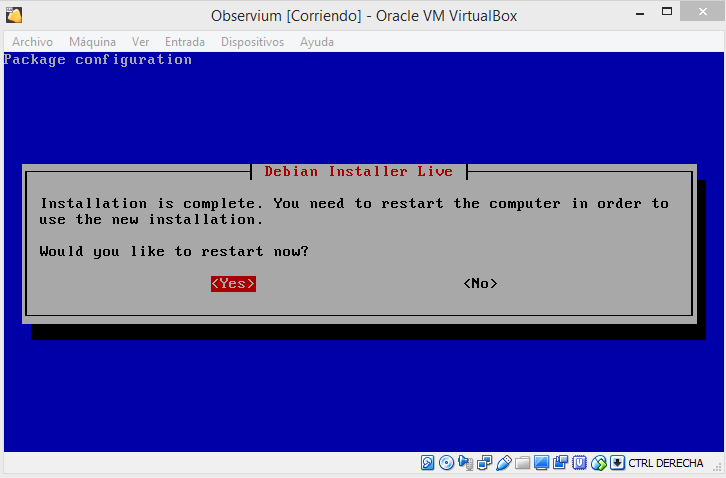
\includegraphics[width=.5 \textwidth]{../images/1-Observium.png}
		\caption{Finalización de la instalación del S.O .}
		\label{image:fin}
\end{figure}
\FloatBarrier

Posteriormente se requiere ingresar un usuario con contraseña , después solo será necesario poner  \textbf{Skip} a las acciones para que al final nos encontremos con la  \textbf{dirección ip} que fue asignada.
 \textbf{Nota: Es importante saber que la dirección ip varía dependiendo de la red a la que se encuentre conectada la máquina virtual}, esto se puede visualizar en la figura \ref{image:ip}.

\FloatBarrier
\begin{figure}[htbp!]
		\centering
		    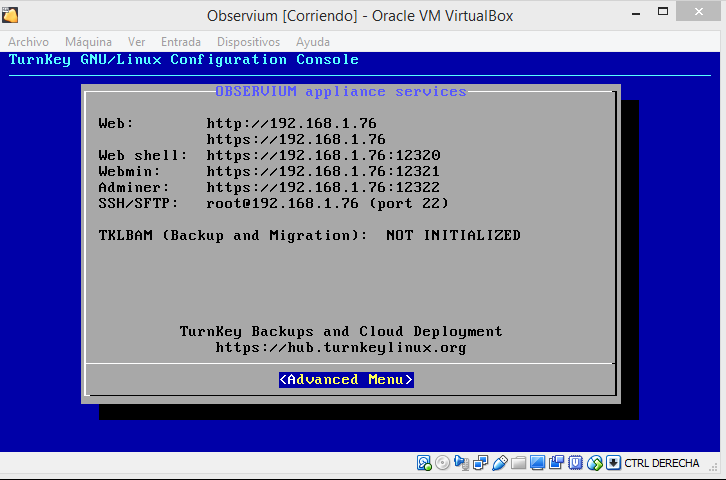
\includegraphics[width=.5 \textwidth]{../images/2-Observium.png} 
		\caption{Asignación de dirección IP.}
		\label{image:ip}
\end{figure}
\FloatBarrier

En este momento podemos decir que ya terminamos el punto de las configuraciones y tenemos a nuestro \textbf{Gestor}.
Si  se quiere comprobar la  conectividad se abre el navegador de nuestro SO nativo y se ingresa la \textbf{dirección IP} que muestra Observium e ingresamos en modo \textbf{administrador} con la contraseña que se  introdujo al inicio de la configuración \ref{image:observium}.

\FloatBarrier
\begin{figure}[htbp!]
		\centering
			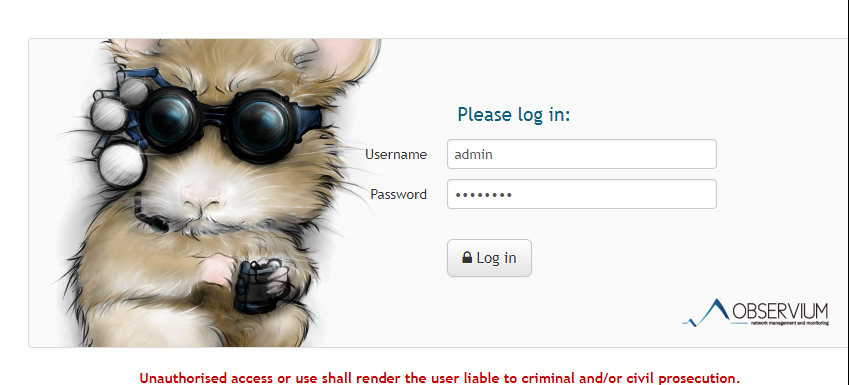
\includegraphics[width=.5 \textwidth]{../images/3-Observium.png}
		\caption{Pág. de Observium}
		\label{image:observium}
\end{figure}
\FloatBarrier

Como se observa en la pagina no se tiene ninguna conectividad de los agentes, esto debido a que no se han regitrado en Observium \ref{image:pag}.

\FloatBarrier
\begin{figure}[htbp!]
		\centering
			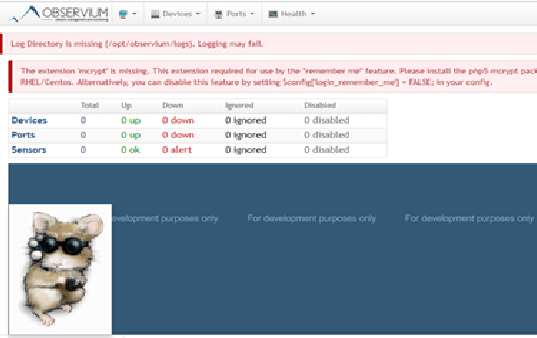
\includegraphics[width=.7 \textwidth]{../images/4-Observium.png}
		\caption{Conectividad}
		\label{image:pag}
\end{figure}
\FloatBarrier

Para poder agregar un agente en Observium solo se necesita poner en la consola el comando \textbf{nano /etc/hosts} con esto ingresamos a nuestro editor de texto nano y solo ingresamos la direccion ip de nuestros sistemas operativos y el nombre de la comunidad que le asignamos a cada so \ref{image:agente}.

\FloatBarrier
\begin{figure}[htbp!]
		\centering
			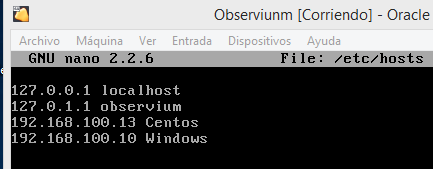
\includegraphics[width=.5 \textwidth]{../images/5-Observium.png}
		\caption{Agentes que contiene Observium}
		\label{image:agente}
\end{figure}
\FloatBarrier

Una vez finalizado todo este procedimeitno, tenemos listo el so Observium como agente.
